\documentclass[10pt, aspectratio=169]{beamer}
\usepackage{siunitx}
\usepackage[T1]{fontenc}
\usepackage{booktabs}
\usepackage[backend=biber]{biblatex}
\usepackage{mathtools,amssymb}
\usepackage{physics}
\usepackage{slashed}
\usepackage{tikz}
\usepackage{tikz-feynman}
\usepackage[list=true, font=small,
labelformat=brace, position=top]{subcaption}
% \setbeameroption{show notes on second screen} %
\addbibresource{thesis.bib}
\graphicspath{ {figs/} }
\usepackage{animate}
\newfontfamily\DejaSans{DejaVu Sans}
\usetheme{Antibes}
% \usepackage{eulerpx}
\usepackage{ifdraft}

% \usefonttheme[onlymath]{serif}
\setbeamertemplate{itemize items}[default]
\setbeamertemplate{enumerate items}[default]
\AtBeginSection[]
{
   \begin{frame}
       \tableofcontents[currentsection]
   \end{frame}
}

\setbeamertemplate{footline}[frame number]
\setbeamertemplate{note page}[plain]
\setbeamertemplate{bibliography item}{\insertbiblabel} %% Remove book
                                %% symbol from references and add
                                %% number

\sisetup{separate-uncertainty = true}
% Macros

%% qqgg
\newcommand{\qqgg}[0]{q\bar{q}\rightarrow\gamma\gamma}

%% ppgg
\newcommand{\ppgg}[0]{pp\rightarrow\gamma\gamma}

%% Momenta and Polarization Vectors convenience
\DeclareMathOperator{\ps}{\slashed{p}}

\DeclareMathOperator{\pe}{\varepsilon}
\DeclareMathOperator{\pes}{\slashed{\pe}}

\DeclareMathOperator{\pse}{\varepsilon^{*}}
\DeclareMathOperator{\pses}{\slashed{\pe}^{*}}

%% Spinor convenience
\DeclareMathOperator{\us}{u}
\DeclareMathOperator{\usb}{\bar{u}}

\DeclareMathOperator{\vs}{v}
\DeclareMathOperator*{\vsb}{\overline{v}}

%% Center of Mass energy
\DeclareMathOperator{\ecm}{E_{\text{CM}}}

%% area hyperbolicus
\DeclareMathOperator{\artanh}{artanh}
\DeclareMathOperator{\arcosh}{arcosh}

%% Fast Slash
\let\sl\slashed

%% Notes on Equations
\newcommand{\shorteqnote}[1]{ &  & \text{\small\llap{#1}}}

%% Typewriter Macros
\newcommand{\sherpa}{\texttt{Sherpa}}
\newcommand{\rivet}{\texttt{Rivet}}
\newcommand{\vegas}{\texttt{VEGAS}}
\newcommand{\lhapdf}{\texttt{LHAPDF6}}
\newcommand{\scipy}{\texttt{scipy}}

%% Sherpa Versions
\newcommand{\oldsherpa}{\texttt{2.2.10}}
\newcommand{\newsherpa}{\texttt{3.0.0} (unreleased)}

%% Special Names
\newcommand{\lhc}{\emph{LHC}}

%% Expected Value and Variance
\newcommand{\EX}[1]{\operatorname{E}\qty[#1]}
\newcommand{\VAR}[1]{\operatorname{VAR}\qty[#1]}

%% Uppercase Rho
\newcommand{\Rho}{P}

%% Transverse Momentum
\newcommand{\pt}[0]{p_\mathrm{T}}

%% Sign Function
\DeclareMathOperator{\sign}{sgn}

%% Stages
\newcommand{\stone}{\texttt{LO}}
\newcommand{\sttwo}{\texttt{LO+PS}}
\newcommand{\stthree}{\texttt{LO+PS+pT}}
\newcommand{\stfour}{\texttt{LO+PS+pT+Hadr.}}
\newcommand{\stfive}{\texttt{LO+PS+pT+Hadr.+MI}}

%% GeV
\newcommand{\gev}[1]{\SI{#1}{\giga\electronvolt}}

%% Including plots
\newcommand{\plot}[2][,]{%
  \includegraphics[draft=false,#1]{./figs/#2.pdf}}
\newcommand{\rivethist}[2][,]{%
  \includegraphics[draft=false,width=\textwidth,#1]{./figs/rivet/#2.pdf}}

%% Including Results
\newcommand{\result}[1]{\input{./results/#1}\!}

\title{A Study of Monte Carlo Methods and their Application to
  Diphoton Production at the Large Hadron Collider}
\subtitle{Bachelorvortrag}
\author{Valentin Boettcher}
\beamertemplatenavigationsymbolsempty

\begin{document}
\hypersetup{pageanchor=false}
\maketitle

\hypersetup{pageanchor=true} \pagenumbering{arabic}

\begin{frame}
  \tableofcontents
\end{frame}

\section{Introduction}
\begin{frame}{Motivation}
  \begin{block}{Monte Carlo Methods}
    \begin{itemize}
    \item (most) important numerical tools (not just) in particle
      physics
    \item crucial interface of theory and experiment
    \item enable precision predictions within and beyond SM
    \end{itemize}
  \end{block}
  \pause
  \begin{block}{Diphoton Process \(\qqgg\)}
    \begin{itemize}
    \item simple QED process, calculable by hand
    \item higgs decay channel: \(H\rightarrow \gamma\gamma\)
      \begin{itemize}
      \item instrumental in its
        discovery~\cite{Aad:2012tfa,Chatrchyan:2012ufa}
      \end{itemize}
    \item dihiggs decay \(HH\rightarrow b\bar{b}\gamma\gamma\)
      \begin{itemize}
      \item process of recent interest~\cite{aaboud2018:sf}
      \end{itemize}
    \end{itemize}
  \end{block}
\end{frame}

\section{Calculation of the \(\qqgg\) Cross Section}
\subsection{Approach}
\begin{frame}
  \begin{columns}[T]
    \begin{column}{.5\textwidth}
      \begin{figure}[ht]
        \centering
        \begin{subfigure}[c]{.28\textwidth}
          \centering
          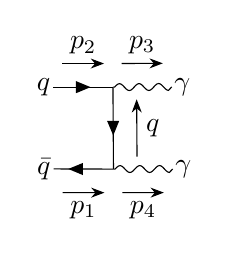
\begin{tikzpicture}[scale=.6]
            \begin{feynman}
              \diagram [small,horizontal=i2 to a] { i2
                [particle=\(q\)] -- [fermion, momentum=\(p_2\)] a --
                [fermion, reversed momentum=\(q\)] b, i1
                [particle=\(\bar{q}\)] -- [anti fermion,
                momentum'=\(p_1\)] b, i2 -- [opacity=0] i1, a --
                [photon, momentum=\(p_3\)] f1 [particle=\(\gamma\)], b
                -- [photon, momentum'=\(p_4\)] f2
                [particle=\(\gamma\)], f1 -- [opacity=0] f2, };
            \end{feynman}
          \end{tikzpicture}
          \subcaption{u channel}
        \end{subfigure}
        \begin{subfigure}[c]{.28\textwidth}
          \centering
          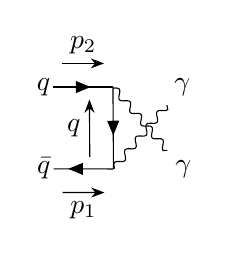
\begin{tikzpicture}[scale=.6]
            \begin{feynman}
              \diagram [small,horizontal=i2 to a] { i2
                [particle=\(q\)] -- [fermion, momentum=\(p_2\)] a --
                [fermion, reversed momentum'=\(q\)] b, i1
                [particle=\(\bar{q}\)] -- [anti fermion,
                momentum'=\(p_1\)] b, i2 -- [opacity=0] i1, a --
                [draw=none] f2 [particle=\(\gamma\)], b -- [draw=none]
                f1 [particle=\(\gamma\)], f1 -- [opacity=0] f2, };
              \diagram* { (a) -- [photon] (f1), (b) -- [photon] (f2),
              };
            \end{feynman}
          \end{tikzpicture}
          \subcaption{\label{fig:qqggfeyn2}t channel}
        \end{subfigure}
%
        \caption{Leading order diagrams for \(\qqgg\).}%
        \label{fig:qqggfeyn}
      \end{figure}
    \end{column}
    \pause
    \begin{column}{.5\textwidth}
      \begin{block}{Task: calculate \(\abs{\mathcal{M}}^2\)}
        \begin{enumerate}[<+->]
        \item translate diagrams to matrix elements
        \item use Casimir's trick to average over spins
        \item use completeness relation to sum over photon
          polarizations
        \item use trace identities to compute the absolute square
        \item simplify with trigonometric identities
        \end{enumerate}
      \end{block}
      \pause Here: Quark masses neglected.
    \end{column}
  \end{columns}
\end{frame}

\subsection{Result}

\begin{frame}
  \begin{equation}
    \label{eq:averagedm_final}
    \langle\abs{\mathcal{M}}^2\rangle = \frac{4}{3}(gZ)^4
    \cdot\frac{1+\cos^2(\theta)}{\sin^2(\theta)} =
    \frac{4}{3}(gZ)^4\cdot(2\cosh(\eta) - 1)
  \end{equation}
  %
  \pause
  \[\overset{\text{Golden Rule}}{\implies}\]
  \pause
  \begin{equation}
    \label{eq:crossec}
    \dv{\sigma}{\Omega} =
    \frac{1}{2}\frac{1}{(8\pi)^2}\cdot\frac{\abs{\mathcal{M}}^2}{\ecm^2}\cdot\frac{\abs{p_f}}{\abs{p_i}}
    = \underbrace{\frac{\alpha^2Z^4}{6\ecm^2}}_{\mathfrak{C}}\frac{1+\cos^2(\theta)}{\sin^2(\theta)}
  \end{equation}

  \pause
  \begin{figure}[ht]
    \centering
    \begin{minipage}[c]{0.3\textwidth}
      \plot[scale=.6]{xs/diff_xs}
    \end{minipage}
    \begin{minipage}[c]{0.3\textwidth}
      \caption{The differential cross section as a function of the
        polar angle \(\theta\).}
    \end{minipage}
  \end{figure}
\end{frame}

\begin{frame}{Comparison with \sherpa~\cite{Bothmann:2019yzt}}
  \begin{itemize}

  \item<1-> choose \result{xs/python/eta} and \result{xs/python/ecm}
    and integrate XS
    \begin{equation}
      \label{eq:total-crossec}
      \sigma = {\frac{\pi\alpha^2Z^4}{3\ecm^2}}\cdot\qty[\tanh(\eta_2) - \tanh(\eta_1) + 2(\eta_1
      - \eta_2)]
    \end{equation}
  \item<2-> analytical result: \result{xs/python/xs}
  \item<3-> compatible with \sherpa: \result{xs/python/xs_sherpa}
  \end{itemize}
  \begin{figure}[ht]
    \centering
    \begin{minipage}[c]{0.3\textwidth}
      \plot[scale=.5]{xs/total_xs}
    \end{minipage}
    \begin{minipage}[c]{0.3\textwidth}
      \caption{\label{fig:totxs} The cross section of the process for
        a pseudo-rapidity integrated over \([-\eta, \eta]\).}
    \end{minipage}
  \end{figure}
\end{frame}

\section{Monte Carlo Methods}

\note[itemize]{
\item Gradually bring in knowledge through distribution.  }
\begin{frame}
  \begin{block}{Basic Ideas}
    \begin{itemize}
    \item<+-> Given some unknown function
      \(f\colon \vb{x}\in\Omega\subset\mathbb{R}^n\mapsto\mathbb{R}\)
      \ldots
    \item<+-> \ldots\ how do we answer questions about \(f\)?
    \end{itemize}
    \;\;\onslide<+->{\(\implies\) Sample it at random points.}
  \end{block}
  \pause
  \begin{block}{Main Applications}
    \begin{enumerate}
    \item<+-> integrate \(f\) over some volume \(\Omega\)
    \item<+-> treat \(f\) as distribution and take random samples
    \end{enumerate}
  \end{block}
\end{frame}

\subsection{Integration}
\note[itemize]{
\item omitting details (law of big numbers, central limit theorem)
\item at least three angles of attack
\item some sort of importance sampling, volume: stratified sampling }
\begin{frame}
  \begin{itemize}
  \item<+-> we have:
    \(f\colon \vb{x}\in\Omega\subset\mathbb{R}^n\mapsto\mathbb{R}\)
    and \(\rho\colon \vb{x}\in\Omega\mapsto\mathbb{R}_{> 0}\) with
    \(\int_{\Omega}\rho(\vb{x})\dd{\vb{x}} = 1\).
  \item<+-> we seek:
    \begin{equation}
      \label{eq:baseintegral}
      I = \int_\Omega f(\vb{x}) \dd{\vb{x}}
      \onslide<+->{= \int_\Omega
        \qty[\frac{f(\vb{x})}{\rho(\vb{x})}] \rho(\vb{x}) \dd{\vb{x}} = \EX{\frac{F}{\Rho}}}
    \end{equation}
  \item<+-> numeric approximation:
    \begin{equation}
      \label{eq:approxexp}
      \EX{\frac{F}{\Rho}} \approx
      \frac{1}{N}\sum_{i=1}^N\frac{f(\vb{x_i})}{\rho(\vb{x_i})}
      \xrightarrow{N\rightarrow\infty} I
    \end{equation}
  \item<+-> error approximation:
    \begin{align}
      \sigma_I^2 &= \frac{\textcolor<+->{red}{\sigma^2}}{\textcolor<.->{blue}{N}} \\
      \sigma^2 &= \VAR{\frac{F}{\Rho}} = \int_{\textcolor<+(3)->{blue}{\Omega}} \qty[I -
                 \frac{f(\vb{x})}{\textcolor<+->{blue}{\rho(\vb{x})}}]^2
                 \textcolor<.->{blue}{\rho(\vb{x})} \textcolor<+->{blue}{\dd{\vb{x}}} \approx \frac{1}{N - 1}\sum_i \qty[I -
                 \frac{f(\vb{x_i})}{\rho(\vb{x_i})}]^2  \label{eq:varI-approx}
    \end{align}
  \end{itemize}
\end{frame}

\begin{frame}{Change of Variables}
  Choose \(\rho(\vb{x}) = \frac{1}{\abs{\Omega}}\)
  \onslide<2->{\(\implies I=\frac{\abs{\Omega}}{N}\sum_{i=1}^N
    f(\vb{x_i})=\abs{\Omega}\cdot\bar{f}\) and
    \(\VAR{\frac{F}{P}}\approx\frac{\abs{\Omega}^2}{N-1}\sum_{i}\qty[f(\vb{x}_i)
    - \bar{f}]^2\)}
  \begin{block}{Results}
    \begin{itemize}
    \item<3-> integrating \(\dv{\sigma}{\theta}\) with target error of
      \(\sigma = \SI{1e-3}{\pico\barn}\) takes
      \result{xs/python/xs_mc_N} samples
    \item<4-> integrating \(\dv{\sigma}{\eta}\) takes just
      \result{xs/python/xs_mc_eta_N} samples
    \end{itemize}
  \end{block}
  \begin{figure}[hb]
    \centering \onslide<3->{
      \begin{subfigure}[c]{.4\textwidth}
        \centering \plot[scale=.6]{xs/xs_integrand}
      \end{subfigure}
    } \onslide<4->{
      \begin{subfigure}[c]{.4\textwidth}
        \centering \plot[scale=.6]{xs/xs_integrand_eta}
      \end{subfigure}
    }
  \end{figure}
\end{frame}

\note[itemize]{
\item proposed by G. Peter Lepage (slac) 1976
\item own implementation!!!
}
\begin{frame}{\vegas\ Algorithm \cite{Lepage:19781an}}

  \begin{columns}
    \begin{column}{.5\textwidth}
      \begin{block}{Idea}
        \begin{enumerate}
        \item subdivide integration volume into grid, take equal
          number of samples in each hypercube \(\iff\) define \(\rho\)
          as step function
        \item iteratively approximate optimal \(\rho = f(\vb{x})/I\)
          with step function
        \item this is quite efficient when \(n\geq 4\)
        \end{enumerate}
      \end{block}
      \pause
      \begin{block}{Result}
        Total function evaluations:
        \result{xs/python/xs_mc_θ_vegas_N}\\
        (for same accuracy as before)
      \end{block}
    \end{column}
    \begin{column}{.5\textwidth}
      \begin{figure}[ht]
        \centering \plot[scale=.6]{xs/xs_integrand_vegas}
        \caption{\(2\pi\dv{\sigma}{\theta}\) scaled to increments
          found by \vegas}
      \end{figure}
    \end{column}
  \end{columns}
\end{frame}

\subsection{Sampling}

\note[itemize]{
\item prop. to density
\item generalization to n dim is easy
\item idea -> cumulative propability the same
}
\begin{frame}
  \begin{itemize}[<+->]
  \item we have: \(f\colon x\in\Omega\mapsto\mathbb{R}_{>0}\)
    (choose \(\Omega = [0, 1]\)) and uniformly random samples \(\{x_i\}\)
  \item we seek: a sample \(\{y_i\}\) distributed according to \(f\)
  \end{itemize}
  \begin{block}<+->{Basic Idea}
    \begin{itemize}[<+->]
    \item<.-> let \(x\) be sample of uniform distribution, solve
      \[\int_{0}^{y}f(x')\dd{x'} = x\cdot\int_0^1f(x')\dd{x'} =
        x\cdot A\] for y to obtain sample of \(f/A\)
    \item let \(F\) be the antiderivative of \(f\), then
      \(y=F^{-1}(x\cdot A + F(0))\)
      \begin{itemize}
      \item sometimes analytical form available
      \item otherwise tackle that numerically
      \end{itemize}
    \end{itemize}
  \end{block}
\end{frame}

\begin{frame}{Hit or Miss}
  \centering
  \animategraphics[loop,scale=.4,autoplay,palindrome]{5}{pi/pi-}{0}{9}
\end{frame}

\begin{frame}{Hit or Miss}
  \begin{block}{Basic Idea}
    \begin{itemize}[<+->]
    \item take samples \({x_i}\) distributed according to \(g/B\),
      where \(B=\int_0^1g(x)\dd{x}\) and
      \(\forall x\in\Omega\colon g(x)\geq f(x)\)
    \item accept each sample with the probability~\(f(x_i)/g(x_i)\)
      (importance sampling)
    \item total probability of accepting a sample: \(\mathfrak{e} =
      A/B < 1\) (efficiency)
    \item simplest choice \(g=\max_{x\in\Omega}f(x)=f_{\text{max}}\)
    \item again: efficiency gain through reduction of variance
    \end{itemize}
  \end{block}

  \begin{block}<+->{Results with \(g=f_{\text{max}}\)  }
    \begin{itemize}[<+->]
    \item<.-> sampling \(\dv{\sigma}{\cos\theta}\):
      \result{xs/python/naive_th_samp}
    \item sampling \(\dv{\sigma}{\cos\theta}\):
      \result{xs/python/eta_eff}
    \end{itemize}
  \end{block}
\end{frame}

\begin{frame}{Hit or Miss}
  \begin{columns}
    \begin{column}{.4\textwidth}
      \begin{block}<+->{Results with \(g=a\cdot x^2 + b\)} Modest
        efficiency gain: \result{xs/python/tuned_th_samp}
      \end{block}
      \begin{itemize}
      \item<+-> Of course, we can use \vegas\ to provide a better \(g\).
      \end{itemize}
    \end{column}
    \begin{column}{.6\textwidth}
      \begin{figure}[ht]
        \centering \plot[scale=.8]{xs_sampling/upper_bound}
        \caption{The distribution \(\dv{\sigma}{\cos\theta}\) and an
          upper bound of the form \(a + b\cdot x^2\).}
      \end{figure}
    \end{column}
  \end{columns}
\end{frame}

\begin{frame}{Stratified Sampling}
  \begin{block}{Basic Idea}
    \begin{itemize}
    \item subdivide sampling volume \(\Omega\) into \(K\) subvolumes
      \(\Omega_i\)
    \item let \(A_i = \int_{\Omega_i}f(x)\dd{x}\)
    \item take \(N_i=A_i \cdot N\) samples in each subvolume
    \item efficiency is given by:
      \(\mathfrak{e} = \frac{\sum_i A_i}{\sum_i A_i/\mathfrak{e}_i}\)
    \end{itemize}
    \(\implies\) can optimize in each subvolume independently
  \end{block}
  How do choose the \(\Omega_i\)? \pause {\huge\vegas! :-)}
\end{frame}

\note[itemize]{
\item no need to know the jacobian ;)
}
\begin{frame}{Observables}
  \begin{itemize}
  \item we want: distributions of other observables
  \item turns out: simpliy piping samples \(\{x_i\}\) through a map
    \(\gamma\colon\Omega\mapsto\mathbb{R}\) is enough
  \end{itemize}
  \begin{figure}[p]
    \centering

  \begin{subfigure}[b]{.49\textwidth}
    \centering \plot[scale=.5]{xs_sampling/histo_sherpa_eta}
    \caption{histogram of the pseudo-rapidity
      (\(\eta\)).}
  \end{subfigure}
  \begin{subfigure}[b]{.49\textwidth}
    \centering \plot[scale=.5]{xs_sampling/histo_sherpa_pt}
    \caption{histogram of the transverse momentum
      (\(\pt\))}
  \end{subfigure}
\end{figure}
\end{frame}

\begin{frame}[allowframebreaks]
  \frametitle{References}
  \printbibliography
\end{frame}

\appendix
\section{Appendix}

\subsection{More on \vegas}

\begin{frame}{\vegas Details}
  \begin{columns}
    \begin{column}{.6\textwidth}
      \begin{block}{Algorithm 1D}
        \begin{enumerate}
        \item start with \(N\) evenly spaced increments
          \(\{[x_i, x_{i+1}]\}_{i\in\overline{1,N}}\)
        \item calculate the integral weights
          \(w_i = \abs{\int_{x_i}^{x_{i+1}}f(x)\dd{x}}\) and define
          \(W=\sum_iw_i\)
          \begin{itemize}
          \item this is done with ordinary MC integration
          \end{itemize}
        \item calculate subdivide the \(i\)-th increment into
          \(K\frac{w_i}{W}\) increments (round up), where
          \(K = \mathcal{O}(1000)\)
        \item amalgamate the new increments into \(N\) groups \(=\)
          new increments
        \end{enumerate}
      \end{block}
    \end{column}
    \pause
    \begin{column}{.4\textwidth}
      \begin{block}{Advantages}
        \begin{itemize}
        \item number of \(f\) evaluations independent of number of
          hypercubes
        \item adaption itself is adaptive
        \item \textcolor{red}{the advantages only show if \(n\)
            ``high''.}
        \end{itemize}
      \end{block}
    \end{column}
  \end{columns}
\end{frame}

\begin{frame}
  \begin{figure}[ht]
    \centering \plot[scale=.9]{xs/xs_integrand_vegas}
    \caption{\(2\pi\dv{\sigma}{\theta}\) scaled to increments found by
      \vegas}
  \end{figure}
\end{frame}
\begin{frame}{\vegas\ + Hit or Miss}
\begin{figure}[ht]
  \centering
  \begin{subfigure}{.49\textwidth}
    \centering
    \plot[scale=.8]{xs_sampling/vegas_strat_dist}
    \caption[The distribution for \(\cos\theta\), derived from the
    differential cross-section and the \vegas-weighted
    distribution]{\label{fig:vegasdist} The distribution for
      \(\cos\theta\) and the \vegas-weighted
      distribution.}
  \end{subfigure}
  \begin{subfigure}{.49\textwidth}
    \centering
    \plot[scale=.8]{xs_sampling/vegas_rho}
    \caption[The weighting distribution generated by
    \vegas.]{\label{fig:vegasrho} The weighting distribution generated
      by \vegas. It is clear, that it closely follows the original
      distribution.}
  \end{subfigure}
  \caption{\label{fig:vegas-weighting} \vegas-weighted distribution
    and weighting distribution.}
\end{figure}
\end{frame}
\end{document}
